\documentclass[12pt, twoside]{article}
\usepackage[letterpaper, margin=1in, headsep=0.2in]{geometry}
\setlength{\headheight}{0.6in}
%\usepackage[english]{babel}
\usepackage[utf8]{inputenc}
\usepackage{microtype}
\usepackage{amsmath}
\usepackage{amssymb}
%\usepackage{amsfonts}
\usepackage{siunitx} %units in math. eg 20\milli\meter
\usepackage{yhmath} % for arcs, overparenth command
\usepackage{tikz} %graphics
\usetikzlibrary{quotes, angles}
\usepackage{graphicx} %consider setting \graphicspath{{images/}}
\usepackage{parskip} %no paragraph indent
\usepackage{enumitem}
\usepackage{multicol}
\usepackage{venndiagram}

\usepackage{fancyhdr}
\pagestyle{fancy}
\fancyhf{}
\renewcommand{\headrulewidth}{0pt} % disable the underline of the header
\raggedbottom
\hfuzz=2mm %suppresses overfull box warnings

\usepackage{hyperref}

\fancyhead[LE]{\thepage}
\fancyhead[RO]{\thepage \\ Name: \hspace{4cm} \,\\}
\fancyhead[LO]{BECA / Dr. Huson / Geometry\\*  Unit 4: Volume and polyhedra \\* 18 October 2022}

\begin{document}

\subsubsection*{4.6 Homework: Volume of cylinders, cones, pyramids, spheres}
\begin{enumerate}
\item The vertices of $\triangle DAN$ have the coordinates $D(-1,-2)$, $A(2,1)$, and $N(-2,3)$, as shown below. Apply the translation $(x,y) \rightarrow (x+5, y+3)$ to $\triangle DAN$. Draw the image $\triangle D'A'N'$ on the set of axes below, labeling the vertices.
\begin{multicols}{2}
  \begin{tikzpicture}[scale=.48]
    \draw [help lines] (-5,-5) grid (10,8);
    \draw [thick, <->] (-5.4,0) -- (10.4,0) node [below right] {$x$};
    \draw [thick, <->] (0,-5.4)--(0,8.4) node [left] {$y$};
    \draw [thick] (-1,-2) node[below] {$D$}--
    (2,1) node[right] {$A$}--
    (-2,3) node[above] {$N$}--
    cycle;
  \end{tikzpicture}\\[0.5cm]
  Which triangle has a larger area, or are they equal in area? Justify your answer.
\end{multicols}

\item What is the volume of a rectangular prism (box) with a base measuring 20 centimeters by 12 cm, and 8 cm tall?  \vspace{2.5cm}

\item What is the volume of an ice cream cone six inches tall and three inches in diameter, \emph{rounded to the nearest whole cubic inch}?  \vspace{3cm}

\item The air traffic control zone above Kennedy airport is approximately a cylinder with a radius of 1 mile and height of 1,000 feet. What is the volume of the zone, \emph{to the nearest whole cubic foot}?

\item Find the area of $\triangle ABC$,  $Area= \frac{1}{2}bh$. The altitude $h$ of the triangle is 3.25 centimeters and the base $AB=6.1$ cm.\\[1cm]
   \begin{tikzpicture}%[scale=0.7]
     \draw [thick]
       (2,0)node[below]{$A$}--
       (8,0)node[below]{$B$}--
       (4,3)node[above]{$C$} --(2,0);
    \draw [dashed] (4,0)--(4,3);
    \draw (4,0)++(0.3,0)--++(0,0.3)--+(-0.3,0);
    \node at (4,1.5)[right]{$h$};
    \node at (5,0)[below]{$6.1$ cm};
  \end{tikzpicture} \vspace{2cm}

\item Find the volume of a pyramid ($V=\frac{1}{3}Bh$) having a height of 2 feet and with a square base having side lengths of 30 inches. Express your result to the \emph{nearest cubic foot}. \vspace{5cm}

\item Find the volume of a hemisphere with a radius of three inches, to the \emph{nearest whole cubic inch}. (The formula for the volume of a \emph{sphere} is $V=\frac{4}{3}\pi r^3$)

\newpage
\item A model rocket is in the shape of a cylinder with a cone-shaped nose cone on top. The diameter of both the cylindrical base and the nose cone is 3 inches. The cylinder section is 12 inches tall and the nose is an additional 3 inches in height. \\[0.5cm]
Find the volume of the rocket, using the formulas for a cylinder of $V=\pi r^2 h$ and a cone of $V=\frac{1}{3} \pi r^2 h$. Round the result to the \emph{nearest whole cubic inch}.  \vspace{8cm}

\item Given a rectangle with area 21, width $x$, and length $x+4$.
  \begin{enumerate}
    \item Find $x$. \vspace{4cm}
    \item Find the perimeter of the rectangle.
  \end{enumerate}

\item Find the volume of a cone having a height of 12 feet and round base with a diameter of 3 feet. Express your result to the \emph{nearest cubic foot}. \vspace{5cm}

\item Find the area of parallelogram $ABCD$. The altitude $h$ of the parallelogram is 4.5 inches and the base $AB=7.15$ in.\\[1cm]
  \begin{tikzpicture}%[scale=0.7]
    \draw [thick]
      (2,0)node[below]{$A$}--
      (8,0)node[below]{$B$}--
      (10,3)node[above]{$C$} --
      (4,3)node[above]{$D$} --(2,0);
  \draw [dashed] (4,0)--(4,3);
  \draw (4,0)++(0.3,0)--++(0,0.3)--+(-0.3,0);
  \node at (4,1.5)[right]{$h$};
  \node at (5,0)[below]{$7.15$ in.};
\end{tikzpicture} \vspace{2cm}

\item Find the volume of a sphere with a radius of 13 inches, to the \emph{nearest whole cubic inch}. \vspace{3cm}

\item Circle $O$ has a radius of 5 inches, and two radii are drawn, $OA$ and $OB$, as shown. The radii are perpendicular, that is, $m\angle AOB=90^\circ$.\\
\begin{tikzpicture}[scale=0.4]
  \draw [thick] (0,0) node[below]{$O$} circle [radius=5];
  \draw [thick] (0,5) node[above]{$B$} --(0,0)--(5,0)node [right]{$A$};
  \draw (0,0)++(0.6,0)--++(0,0.6)--+(-0.6,0);
\end{tikzpicture}
\begin{enumerate}
  \item Find the circumference of circle $O$. \vspace{1.5cm}
  \item Find the length of the arc $\stackrel\frown{AB}$
  \end{enumerate}

        
\newpage
\subsubsection*{Classwork: Circles and angle measures}
\item A round pizza is sliced into five equal slices.
 \begin{center}
 \begin{tikzpicture}
 \draw [thick] (0,0) circle [radius=3cm];
 \draw [fill] (0,0) circle [radius=0.05] node[above right]{$A$};
 \draw [thick] (0,0)--(18:3) node[right]{$B$};
 \draw [thick] (0,0)--(90:3) node[above]{$C$};
 \draw [thick] (0,0)--(162:3);
 \draw [dashed] (0,0)--(234:3) node[below left]{$D$}--(-54:3);
 \draw [thick] (0,0)--(-54:3) node[below right]{$E$};
 \end{tikzpicture}
 \end{center}
 \begin{enumerate}
   \item What is the \emph{central angle} of a slice? (that is, the $m\angle CAB$) \vspace{2cm}
   \item What is the area of the slice? (one-fifth of the pie) \vspace{3cm}
   \item What is the $m\angle ADE$? \vspace{3cm}
 \end{enumerate}

\item Convert $45^\circ$ to radians. (leave your answer in terms of $\pi$) \vspace{1.5cm}

\item Angle $A$ has a measure of 1.2 radians. How much is that in degrees, \emph{rounded to the nearest whole degree}?



\end{enumerate}
\end{document}